\documentclass[A4]{article}

%\usepackage[iso]{umlaute}
%\usepackage{german}
\usepackage{graphicx}
\usepackage{listings}
\usepackage{comment}
\excludecomment{draft}
\setlength{\parindent}{0cm}
\setlength{\columnsep}{25pt}
\sloppy

% Your name
\author{Paul Preissner \\ Technische Universit\"at M\"unchen}

\title{Seminar Advanced Computer Architecture \\
       {\bf Actors}
}

% Date of your talk
\date{06.07.2017}


\begin{document}

\maketitle

\begin{abstract}
The actor model is a programming paradigm developed specifically with concurrent and distributed computing in mind. It defines a system of self-contained actors that only communicate with each other through dedicated messages and adhere to the basic semantic properties of encapsulation, fairness and location transparency. 
This paper will elaborate on the fundamental concepts and aforementioned semantics of the model, discuss the issues of implementation, current practical usage of the model and a brief comparison with other concurrency models. 
\end{abstract}

\section{Introduction}
\label{introduction}
Ever since the introduction of multi-processor systems in the 1970s and multi-core processors in the early 2000s, one of the main topics in computer science has been how these systems can be utilized to their full capacity, depending on the programming language employed. 
Most programming languages have been adapted to enable concurrent computing either natively or through libraries. Since "[c]oncurrency can be solved by a good programmer in many languages, [...] but it's a tough problem to solve" as former Twitter engineer Alex Payne describes \cite[p.~15]{Agha2016:2}, it seems counter-intuitive to use a language originally defined for sequential execution. Therefore in the 1970s research first delved into defining languages and paradigms meant to primarily deal with concurrent computing. One of these paradigms is the actor model, initially developed by Carl Hewitt and his colleagues, formalized by Gul Agha in 1985 and researched by multiple groups and universities since then \cite{reference/parallel/KarmaniA11}. The model is "commonly used to solve concurrency problems, and it makes that problem a lot easier to solve" \cite[p.~15]{Agha2016:2}.
Subsequently, this paper will take a look at the fundamentals and basic semantics of the actor model, followed by a discussion of some issues the model entails in implementation and a look at the potential it offers nowadays, concluded by a brief comparison to other models. 

\section{Fundamentals \& semantics of the Actor model}
\subsection{Fundamental concept}
As mentioned before, the model is based on the message-passing paradigm, which sees communication as the exchange of data/directive messages between whatever is defined as a computational unit. Computation is encapsulated into actors while communication is only conducted via messages. As Agha puts it, the model furthers one key advantage of object-oriented programming, the separation of an object's interface from its representation, and expands it by separation of control from the computational logic \cite{reference/parallel/KarmaniA11}. This allows actor-based programs to be made up of "self-contained, autonomous, interactive, asynchronously operating components" \cite[p.~1]{reference/parallel/KarmaniA11} which makes them ideal for inherently nondeterministic systems such as distributed or mobile networks. 
\subsubsection{Actor}
According to its definition, a faithfully implemented actor can only send messages to actors it already knows. It is not allowed to guess or construct names or addresses of other actors \cite{reference/parallel/KarmaniA11}. Construction of a recipient's identifier would only be allowed if all properties and valid value ranges of the identifier are known. 
Furthermore, an actor by definition may proceed with any and all of three possible actions when receiving a message, given it is idle and ready to compute (as seen in \ref{Actors}): 
\begin{itemize}
\item The actor may send messages to other actors, for example as a reply to the original sender or as subsequent communication to other actors,
\item create new actors for arbitrary purpose, for example as workforce for a certain parallel task,
\item update its local state, in that it may do arbitrary computations within itself.
\end{itemize}
The third action leads to another fundamental restriction of the actor model: an actor can only influence its own local state . It is not allowed to directly change the state of other actors in any way, such changes have to be requested through messages\cite{reference/parallel/KarmaniA11}. This presents a common pitfall where a faithful implementation tends to prove inefficient and is willingly omitted in favor of better performance. 
\begin{figure}
\centerline{
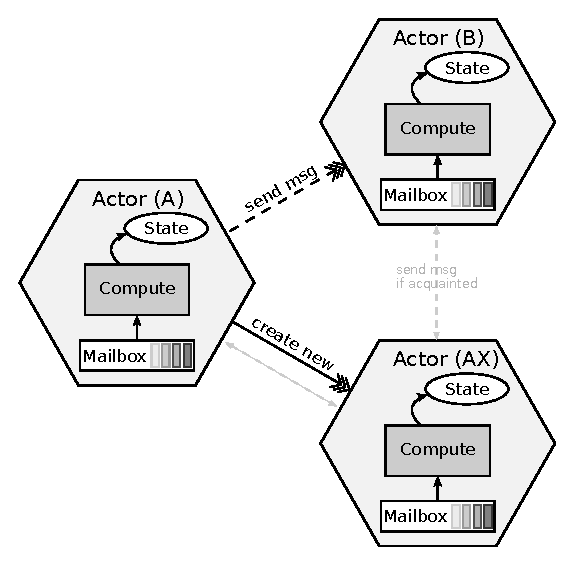
\includegraphics[width=0.8\textwidth]{actorsExample.eps}
}
\caption{Any actor may send messages to other known actors, create new actors or update its own state.}
% A label to allow refering to this figure in the text.
\label{Actors}
\end{figure}

\begin{draft}
\subsubsection{Sample actor program}
Many actor languages and libraries for most common languages exist, most of which are still actively supported or developed, though unfortunately, some of them have imprecise documentation and little developer support.\cite{WikiLang} \\
To illustrate actors, the C++ Actor Framework \cite{cshw-nassp-13}\cite{chs-rapc-16} was used to implement a small Ping Pong program as in listing 1. An actor A sends a string {\it Ping} to an actor B. Actor B replies to any incoming messages matching to {\it Ping} with a reply {\it Pong}. Actor A reacts to any incoming {\it Pong} with yet another {\it Ping}.
The output of this program is therefore a continuous back and forth of {\it Ping} and {\it Pong}. It shows, however, that using actors in programs proves fairly easily given a properly implemented library. Note that no thread management or balancing has to be done by the high level programmer. It is only necessary to specify the behaviors for actors and start a first call on at least one actor. The rest is done almost entirely by the library. This small sample program is scheduled by CAF to utilize all four threads of the executing Intel Core i7-7500U to at least 75\% utilization. 
\begin{lstlisting}[language=C++, caption=sample code, frame=single, breaklines]
[includes, usings]

behavior pong(event_based_actor* self, string selfname) {
  return {
    //if the message contains a string, proceed
    [=](const string& what) -> string {
      aout(self) << selfname << ": " << what << endl;
      // reply Pong
      return string("Pong!");
    }
  };
}

void ping(event_based_actor* self, const actor& buddy, string selfname) {
  // send Ping to buddy (timeout for reply = 10s)
  self->request(buddy, std::chrono::seconds(10), "Ping!").then(
    //if the message contains a string, proceed
    [=](const string& what) {
      aout(self) << selfname << ": " << what << endl;
	  //if reply is as expected, restart ping again
	  if(what.compare("Pong...") == 0)
		  ping(self, buddy, selfname);
    }
  );
}

int main() {
  [caf setup]
  // create a new actor that calls 'pong()'
  auto actor_B = system.spawn(pong, "B");
  // create another actor that calls 'ping(actor_B)';
  auto actor_A = system.spawn(ping, actor_B, "A"); }
\end{lstlisting}
\end{draft}

\subsection{Semantics}
The Actor model has a few major semantic properties. These are "encapsulation and atomic execution of methods (where a method represents computation in response to a message), fairness, and location transparency" \cite[p.~4]{reference/parallel/KarmaniA11} which if enforced almost guarantee correct execution of the model. If not, however, they put the task of checking for faithful implementation onto the programmer. 
\subsubsection{Encapsulation and atomic execution}
Encapsulation describes the previously mentioned property that no actor can directly influence the state of another actor. More precisely, "no two actors share state" \cite[p.~4]{reference/parallel/KarmaniA11} and on a conceptual level change state atomically. An actor upon receiving a message will compute based on the behavior defined within and will not branch into different computations if it receives another message while busy. Faithfully the actor will buffer the pending message, finish its current computation, then continue with the pending message, effectively completing an atomic step. 
Theoretically, for the sake of performance, it makes sense to interrupt current computation and switch to a different task the moment a message arrives or starts to work in parallel, however, this violates the semantic definition of the Actor model, introduces hazards and compounds modeling and checking of the program.
\subsubsection{Fairness}
In Karmani's paper, fairness is the property that "every actor makes progress if it has some computation to do, and [...] every message is eventually delivered [...] unless the destination actor is permanently disabled" \cite[p.~5]{reference/parallel/KarmaniA11}. Due to atomicity, an actor will always compute something if it received a message. 
This notion of fairness assumes that the underlying scheduler is fair as well. 
Given that, one can reason more easily about the liveness properties of a program \cite[p.~5]{reference/parallel/KarmaniA11} as this property guarantees that in a composition of actor systems, no busy system can inhibit the progress of another system thus stall the entire program.
\subsubsection{Location transparency}
One more property of the model is that the actual location of an actor is independent of its identifier. A program can be constructed without the need to know the physical topology of the executing system. This facilitates another property: mobility.
"Mobility is defined as the ability of a computation to migrate across different nodes" \cite[p.~5]{reference/parallel/KarmaniA11}, meaning actors can be shifted across nodes without affecting the correctness of execution. This is key for effective runtime load-balancing of irregular and dynamic applications, energy efficiency optimization, fault-tolerance in case of partial network failure and improved scalability. 

\subsection{Means of synchronization and abstraction}
\subsubsection{Synchronization}
Synchronization in the actor model  has to be handled through messages. Karmani describes a solution based on the same principle as traditional procedure calls, "Remote Procedure Call (RPC)-like messaging" \cite[p.~6]{reference/parallel/KarmaniA11}. A request is sent out by an actor A which then waits. If it receives a matching reply by any actor B, A proceeds. If not, B's message is deferred until the expected reply arrives \cite[p.~6]{reference/parallel/KarmaniA11}. Specific implementation is down to the individual library or language.
RPC-like messages offer themselves as a solution for ordered processing of messages or when all next actions of the requestor depend on the reply. 
Another approach are so-called local synchronization constraints. A set of constraints is defined over an actor that specifies the order it should keep and process messages in, depending on its state and the message type and content. \cite[p.~34]{Agha2016:2}
Alternatively, specialized constructs called {\it synchronizers} can be used to act as a pre-processing of messages that ensures correct order.
Karmani suggests that these approaches can be used to construct patterns like pipelining and divide-and-conquer to map actors to a more complex task distribution in a modular fashion \cite[p.~6]{reference/parallel/KarmaniA11}.
\subsubsection{Abstraction}
Patterns may also be used in a different fashion for abstraction. As Karmani points out, ideally a programmer can utilize a language or library in a fashion similar to the conceptual level of the problem at hand. Instead of treating actors as single actors one would prefer to have abstractions that compose actors in a useful way. \cite[p.~7]{reference/parallel/KarmaniA11}
Patterns can be employed to structure communication, in that groups of actors are assigned properties by which they can be identified or discarded as recipients for certain messages. For example, actors can specify their group and that they are only interested in specific message data. A sender can specify properties the recipients of its message need to satisfy. A message can then be sent out to a satisfying group without performing many individual checks. 

\section{Reality and issues of implementation}
While these semantics are logical in theory, the reality of implementation is different. Not all properties can be implemented faithfully while still performing well without major optimization work. This might lead to programmers attempting to implement an actor language or library to take shortcuts to achieve better performance. But those supposed optimizations might violate the properties and constraints leading to flawed execution. Karmani notes that "a faithful but naive implementation of the Actor model can be highly inefficient" \cite[p.~8]{reference/parallel/KarmaniA11} and may only be feasible for coarse-grained concurrency \cite[p.~7]{conf/pppj/KarmaniSA09} but this "may be addressed by compilation and runtime techniques" \cite[p.~8]{reference/parallel/KarmaniA11}. This chapter will outline a few potential pitfalls and potential solutions.
Note that garbage collection and safe messaging are mentioned by Karmani as yet unresolved issues\cite[p.~10]{conf/pppj/KarmaniSA09}, but will not be discussed here due to lack of clear options for solution.
\subsubsection{Message latency}
Latency is natural to any system, especially distributed ones. The further a message has to travel, the higher the latency between send and receive is. 
Conceptually this is fixed by overlapping communication and computation. This way computation can partially mask the latency. This can still be outweighed by a disproportional surplus of messages, therefore a program needs to be engineered as to not overburden communication. Good overlap also needs suitable decomposition of the program into actors and smart migration. \cite[p.~8]{reference/parallel/KarmaniA11}
Another cruder aspect that may lower latencies is improved network interconnects, be it connections between distributed clients or data buses in embedded systems. 
\subsubsection{Naive send vs channels}
It was previously established that actors may only send messages to actors they know. Some languages and libraries modify this idea towards the concept of channels, specifically with stateful channel contracts, "a protocol that governs the communication between two end-points (actors) of the channel" \cite[p.~8]{reference/parallel/KarmaniA11}. This way the allowed type and order of messages can be specified in a more intuitive way as opposed to individual checks of messages in each actor and additional synchronization. \cite[p.~8]{reference/parallel/KarmaniA11}
\subsubsection{Thread overhead and context switches}
A basic actor language or library might opt for mapping an actor to a thread for simplicity. The issue this presents is overhead due to context switching and thread creation. Every time the program execution switches to a different actor, it has to perform a complete context switch including saving its entire stack, counters and registers. This problem becomes increasingly prevalent the more actors a program uses. Karmani presents one possible solution in continuations based actors which don't perform a full context switch and significantly reduce overhead. In his testing, going from traditional threads to continuations in ActorFoundry reduced runtime of a thread switching benchmark by over 60\% from 695s to 267s. \cite[p.~8]{conf/pppj/KarmaniSA09}
\subsubsection{Deep copies vs referencing}
By definition, an actor may not change the state of another actor directly. Naively on a shared memory system any data exchange would need to happen by copying the data into a message, which is slow compared to sending a reference. Sending a reference however carries the risk of direct changes violating the model in the process. Karmani's optimization efforts suggest allowing immutable types to be sent by reference. According to his numbers in the aforementioned benchmark, sending the main message content type by reference reduced runtime by another 84\%. \cite[p.~9]{conf/pppj/KarmaniSA09}
The speedup achieved this way depends on which message content types are most common in a program as well as the scale of the system.
\subsubsection{Scheduling}
The model claims fairness in that every actor will make progress if it has pending messages. This, however, has to be ensured by the scheduler. It's not inherently an issue but can be if the scheduler does not comply. What Karmani did for his testing was to write a custom scheduler which monitors the worker threads and spawns a new thread when no progress is made yet actors are queuing to be scheduled. While not highly sophisticated, his method when tweaked performs almost identical to the default JVM scheduler but does guarantee fairness. \cite[p.~9]{conf/pppj/KarmaniSA09}

\section{Current usage of actor systems}
\subsubsection{Actors in distributed systems}
There are multiple levels at which the model can be applied in distributed systems. An intuitive option is to model clients as actors and map them 1:1 or cluster several clients into an actor. Communication then maps to the physical links between clients. This may not be efficient or suitable for the application though. A more useful mapping is to decouple and map parts of the program, such as a user of a service or a certain part of a service itself. This is the case for systems such as the {\it Facebook} chat backend \cite{Facebook}, {\it Twitter} message queues \cite{Twitter}, game servers for the video game {\it Halo 4} \cite{Halo4} or the web application framework {\it Lift} \cite[p.~14]{Agha2016:2}. Other projects exist in high performance computing, demonstrated for example by the {\it ActorX10} group of the {\it Invasic} project at TUM which uses a fusion of X10 and the actor model to illustrate how actors can be used to build highly scalable programs while also simplifying communication and separating control flow from computation \cite[p.~4]{Roloff:2016:AAL:2931028.2931033}. 
A similar potential lies in so-called microservices, a type of service-oriented architecture where collections of independent services are composed into a whole application. The idea is to achieve better scalability, decentralized control and fault-tolerance. \cite{MicroS}
\subsubsection{Actors in embedded systems}
The model is also suitable to map programs and algorithms on a very small scale in embedded systems. About actor-oriented design of embedded systems in 2002, Edward A. Lee et al. argue this approach is "particularly effective for system-level design" \cite[p.~12]{Lee03actor-orienteddesign}. Components of the system, such as parts of an algorithm, are modeled as actors to enable better reasoning over execution within the system. The actor model offers them a clear method for abstraction and definition of interfaces, object representations and connections. Lee et al. state that "[t]he primary benefit of actor-oriented design is the possibility of succinctly capturing the requirements of an embedded system by the modeling properties of a model of computation" \cite[p.~23]{Lee03actor-orienteddesign}, specifically satisfying  the requirements of model-based design. 
Contrary to using actors in the design stage, some efforts use the model directly in the implementation of programs. The previously mentioned ActorX10 library illustrates this by implementing an object detection module using an algorithm that features multiple stages. Each stage is modeled as an actor receiving data messages from the previous stage actor and sending its result to the next. This structure can be exploited for parallelism by pipelining. Once a stage is finished with one input, it can immediately work on the next input data. Every stage can have almost 100\% uptime and a final result is had each time the last stage finishes. \cite[p.~4]{Roloff:2016:AAL:2931028.2931033} This could allow even further optimization, for example in hardware through specialized ASICs for certain stages. 
Omer Kilic of the Erlang Solutions group also sees the actor model very suited for current challenges in computing technology such as the creation of complex SoCs, IoT devices and heterogenous architectures \cite[p.~5]{ErlangKilic}.

\section{Versus other models of concurrency}
\subsubsection{vs Petri nets}
Petri nets on a conceptual level are mathematical graph-based models with two types of nodes, places and transitions. Places are equal to conditions of any form while transitions are possible events. Flow within the model is represented by arcs pointing from either a place or a transition to the respective other. The net describes a complex system of pre- and postconditions for possible events. Every such place/condition can have an arbitrary number of tokens which can each trigger a transition and are then "transferred" to the postcondition of that event. \cite{Petri2}\cite{murata1989petri}
This can be exploited for concurrency by placing multiple tokens in the net. 
The largest difference to the actor model appears to be that actors are modeled as the (abstract) computing units themselves with communication between each which can lead to state changes while a petri net describes the possible changes and events mostly independent of the representation of computation.
\subsubsection{vs process calculi}
Process calculi are not one model specifically but a collection of similar formal models. Their basic definitions all include a few key properties. Processes communicate/interact through message-passing, similar to the actor model, however anonymously via channels, unlike the pure actor model. Processes are modeled as a composition of primitives and operators, unlike the actor model which does not specifically model the actions within an actor. These operators are subject to algebraic laws to facilitate reasoning about the system. \cite{Baeten:2005:BHP:1085667.1085669} The partial similarities between the two models do not come as a surprise considering Carl Hewitt named process calculi as one influence on his work. 
\subsubsection{vs input/output automaton}
I/O automata approach the issue of concurrency at an even more modular level. They can be used to model single components of almost any kind, be it computational units, data or communication methods. An automaton is essentially a state machine with inputs, outputs and some sort of internal action. Only the in- and outputs may be used to communicate with other automatons, internals are hidden. \cite{lynch1996distributed}
In this way there is some resemblance to the encapsulation in the actor model, however the actor model does already specify communication and basic actor structure. The automata could in theory be used to model an actor system, however with more effort.
\section{Conclusion}
\label{conclusion}
To summarize, this paper offers a concise overview of actors. It explains the fundamentals of the actor model, the semantic properties encapsulation, fairness and location transparency (and with it mobility), synchronization through RPC-like communication and local constraints, as well as patterns for abstraction. 
It was established that while a faithful implementation of the model is inefficient, several approaches can be taken to optimize runtime behavior in latency masking, sending efficiency and parallelism overhead.
Lastly, current usage of the model was discussed. It's seems very well suited for distributed computing as well as embedded systems as its structures and communication can be nicely mapped to such systems and facilitate correctness checking. 
Other models of concurrency share some properties with the model, yet it stands out with distinct advantages. 
Unfortunately, the extent of this paper does not allow deeper analysis of the model or an expanded view on its usage in modern commercial or free/open source projects as the presented overview hints at a wide range of possible applications. It is clear, however, that it has great potential for parallelizable challenges in computing and more research is needed to materialize this potential.


% Put citations from bibtex into References section which were not
% explicity cited.
\nocite{Agha2016,conf/eef/RenA96,WikiLang}%ActorSander,cshw-nassp-13,Petri1}


\bibliographystyle{plain}
\bibliography{seminarpaper}
\end{document}